In this section we emphasize the importance of covariates for network inference. Accounting for environmental effects changes the structure of all inferred networks we present; nodes with the highest betweenness scores are highlighted to spot these changes. Most frequently, it results in reducing the number of edges (i.e. making the network sparser). However new edges can appear as well, as adjusting for a covariate also reduces the variability, which improves the detection power. In all examples, we used the resampling method described in Section \ref{sec:inference}, which provides edge selection frequencies. Eventually, we have to threshold these frequencies to draw actual networks; the value of the threshold obviously affects the density of the plotted networks (see Fig.~\ref{QETOak}). 


\subsubsection{Fish populations in the Fatala River estuary}
\label{barans}

Networks on Fig.~\ref{baransNets} suggest a predominant role of the \textit{site} covariate compared to the \textit{date}. Indeed, adjusting for the \textit{site} results in much sparser networks (Fig.~\ref{QETOak} in appendix). It deeply modifies the network structure: the \textit{site} network has 12 new edges and only 6 in common with the \textit{null} network. Besides, the  highlighted nodes only change when introducing the \textit{site} covariate.  This suggests that the environmental heterogeneity between the sites has a major effect on the \modif{variations of species abundances}, while the effect of the date of sampling is moderate.



  \begin{figure}[H]
      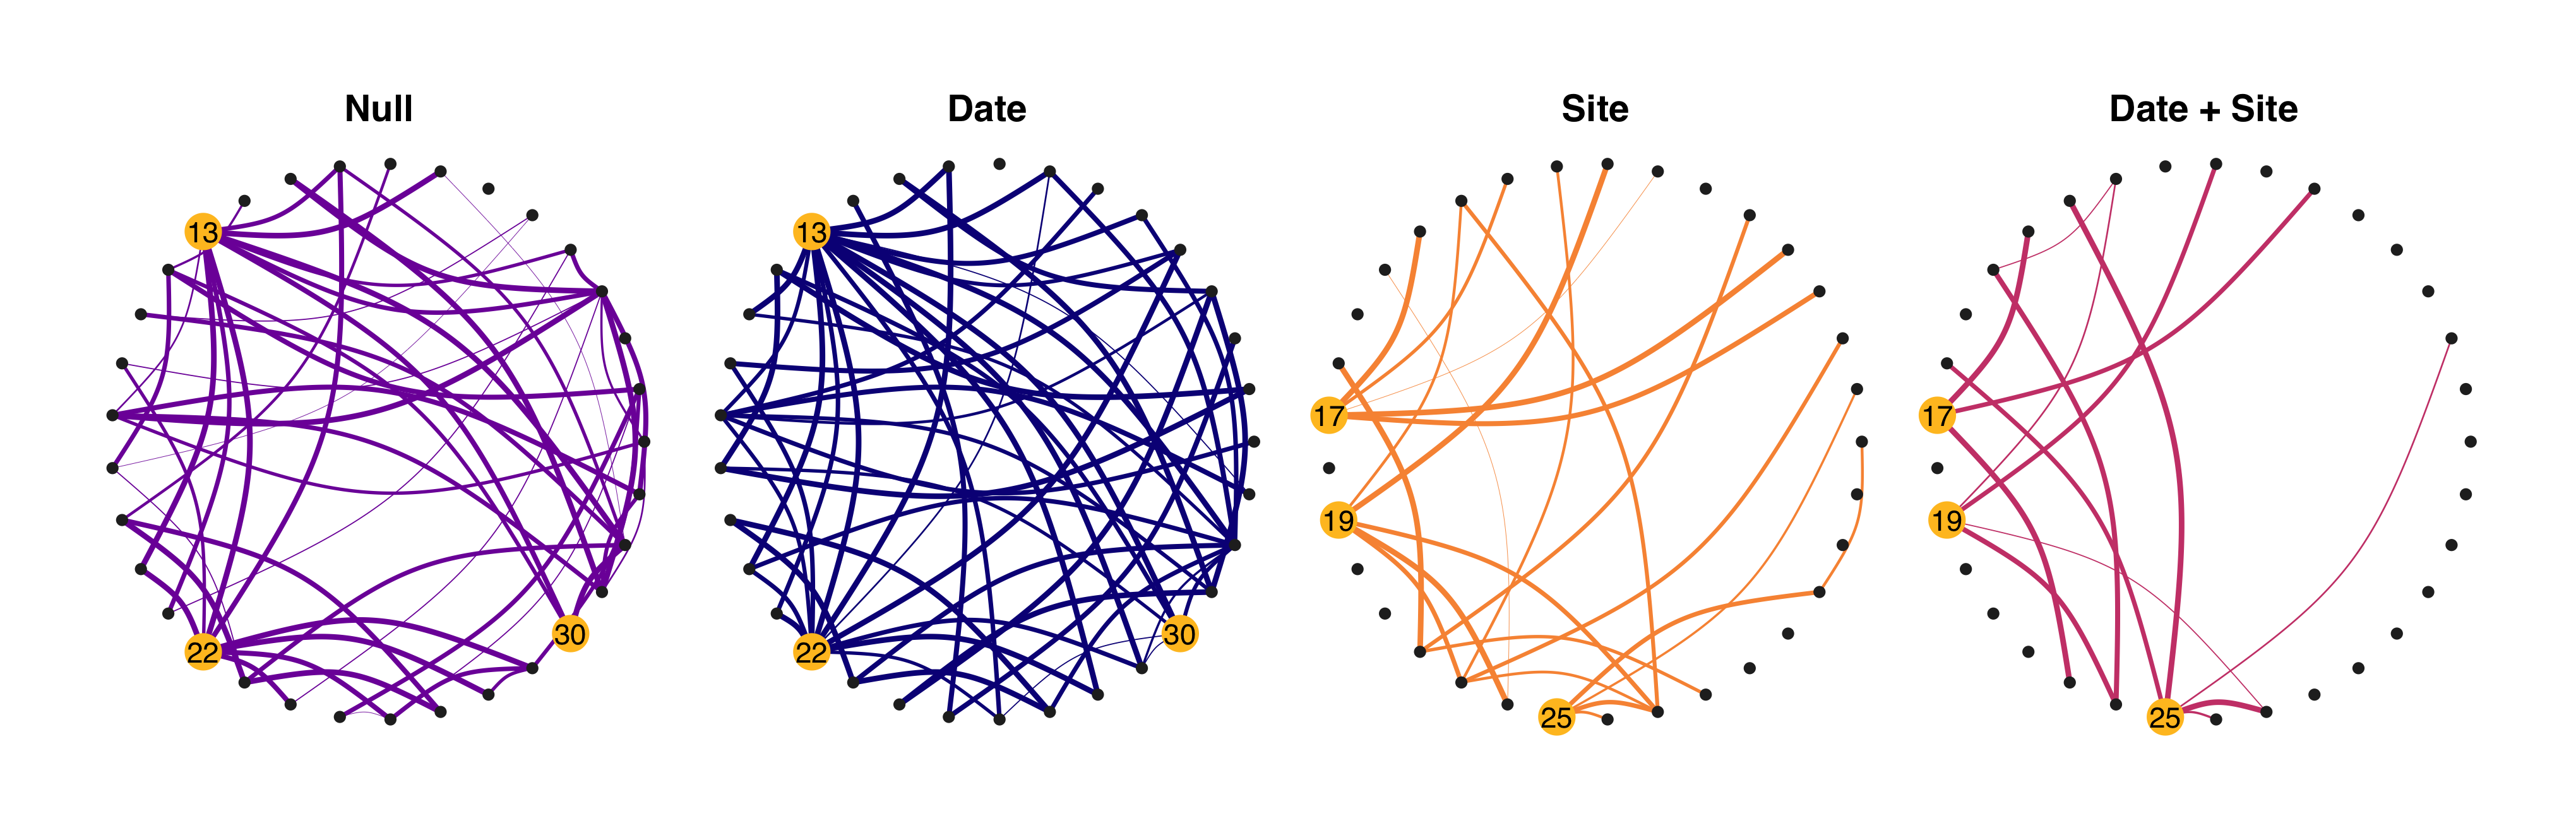
\includegraphics[width=\linewidth]{figs/BaransNets.png}
      \caption{Interaction networks of Fatala River fishes inferred when adjusting for none, both or either one of the covariates among \textit{site} and \textit{date}. Highlighted nodes spot the highest betweenness centrality scores. Widths are proportional to selection frequencies. $S=100$, $f'=90\%$. }
    \label{baransNets}
  \end{figure}
  

%%%%%%%%%%%%%%%%%%%%%%%%%%%%%%%%%
\subsubsection{Oak powdery mildew}  
\label{oak}

When providing the inference with more information (tree status, distances), the structure of the resulting network is significantly modified. Nodes with high betweenness scores differ from one model to another. There is an important gap in density between the \textit{null} model and the others, starting from a $25\%$ selection threshold (Fig.~\ref{QETOak} in appendix). From a more biological point of view, the features of the pathogen node are greatly modified too: its betweenness score is among the smallest in the \textit{null} network (quantile $16\%$), and among the highest in the two other networks (quantiles $93\%$ and $96\%$). Its connections to the other nodes vary as well. 
Accounting for covariates results in less interactions with the pathogen but a greater role of the latter in the pathobiome organization.


 \begin{figure}[H]
    \centering
    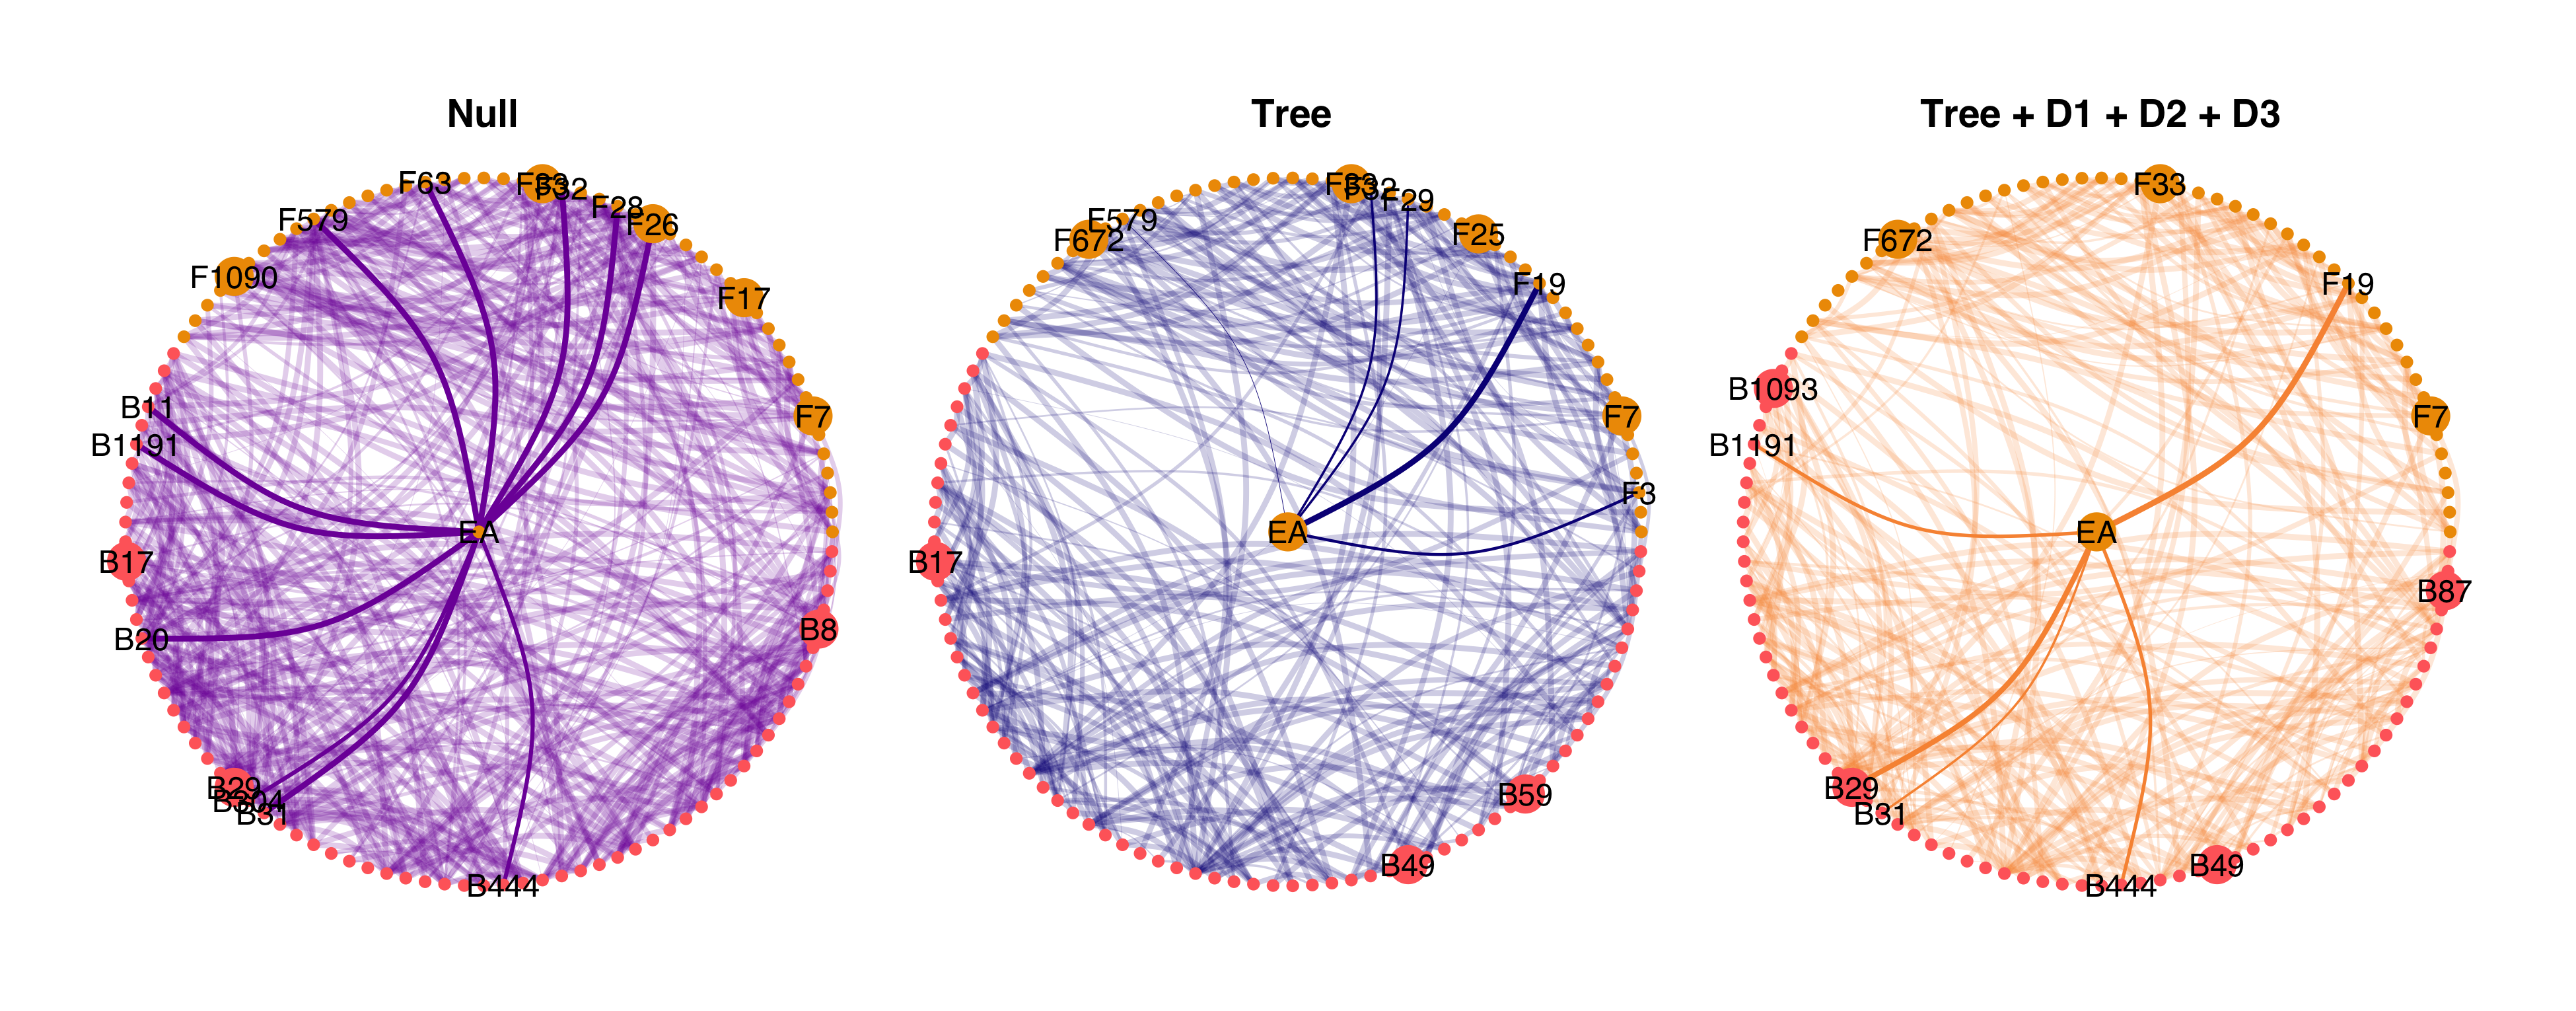
\includegraphics[width=\linewidth]{figs/OakProbNets.png}
    \caption{Pathogen interaction networks on oak leaves inferred with EMtree when adjusting for none, the \textit{tree} covariate or \textit{tree} and distances. Bigger nodes represent OTUs with highest betweenness values, colors differentiate fungal and bacterial OTUs. Widths are proportional to selection frequencies. $S=100$, $f'=90\%$ .  }
    \label{oakNets}
\end{figure}

Using the dataset restricted to infected samples (39 observations for 114 OTUs) and correcting for the leaves position in the tree (proxy for their abiotic environment), \citet{jakuch} identifies a list of 26 OTUs likely to be directly interacting with the pathogen. Running EMtree on the same restricted dataset with the same correction yields a good concordance with  edge selection frequencies, as shown in Fig.~\ref{otujak}.


\begin{figure}[H]
    \centering
    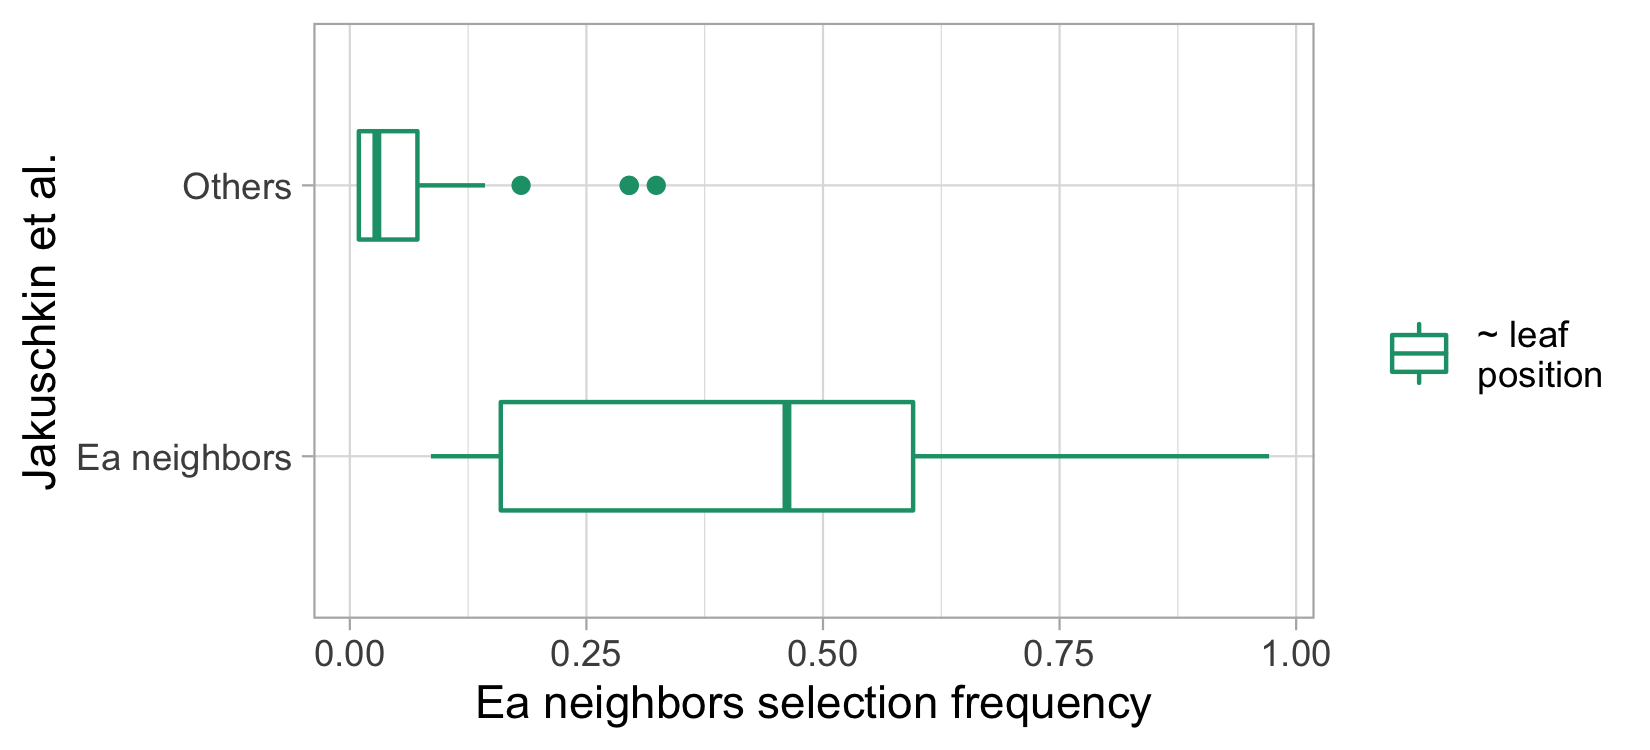
\includegraphics[width=9.5cm]{figs/EAneighbors.png}
    \caption{EMtree selection frequencies of pathogen neighbors compared to \citet{jakuch} results, computed on infected samples and adjusting for the leaf position (100 subs-samples). }
    \label{otujak}
\end{figure}

 
